\section{Strongly connected components (SCC)}
Vi ser på definisjonen av strongly connected components (heretter SCC): \index{SCC (strongly connected components)}
\begin{definition}
Anta at vi har en rettet graf $ G = (V, E) $. Vi har da at en \textbf{SCC} av $ G $ er et maksimalt sett av noder $ U \subseteq V $ slik at for alle $ u_i $, $ u_j \in U $ har vi at $ u_i \leadsto u_j $ og $ u_j \leadsto u_i $.
\end{definition}

Med andre ord: en SCC er en del (partisjon) av grafen der alle nodene i den partisjonen kan nå alle andre noder i partisjonen. Vi ser på et eksempel: \index{graf!partisjon}

\begin{example} Finn alle SCCer i grafen:
\begin{figure}[h!]
\centering
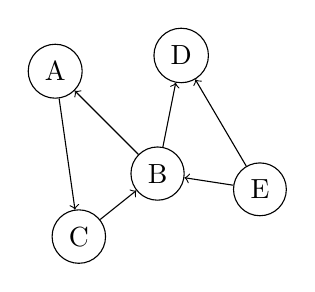
\begin{tikzpicture}[->]
\tikzstyle{v} = [circle, draw=black]
\tikzstyle{e} = [draw=black]

\node[v] (A) at (-1.3, 1.3) {A};
\node[v] (B) at (0, 0) {B};
\node[v] (C) at (-1, -.8) {C};
\node[v] (D) at (0.3, 1.5) {D};
\node[v] (E) at (1.3, -0.2) {E};

\draw[e] (A) to (C);
\draw[e] (C) to (B);
\draw[e] (B) to (A);
\draw[e] (B) to (D);
\draw[e] (E) to (B);
\draw[e] (E) to (D);
\end{tikzpicture}
\end{figure}
Vi ser at \{A, B, C\} danner en SCC. D har ingen kanter ut. Den må derfor være sin egen SCC. E ingen kanter inn, den må også være sin egen SCC. Vi har da at vi kan partisjonere grafen slik: \{\{A, B, C\}, \{D\}, \{E\} \}
\end{example}